%
% Should we compile for the Iliad (ebook reader), or regular A4
%
\newif\ifcompileiliad
	\compileiliadfalse %Iliad (true) or regular A4 (false)?
\newcommand{\TextSize}{13}
\newcommand{\BaseLineSkip}{15}
\newif\ifDownscaledFinalDoc
	\DownscaledFinalDoctrue		% Uib 13pt (true) or Regular 12pt (false)
%
% Compile draft (double line spacing)?
%
\newif\ifDraft
	\Draftfalse		% Draft (true) or Final (false)
% We use the book class
%
\ifcompileiliad
	\documentclass[10pt]{book}
\else
	\documentclass[12pt]{book}
\fi

% Include the set_up
%
% Settings file
%
%=======================================================================
%-------------This file controls various document settings--------------
%=======================================================================


%
% The geometry package allows consistent control of page layout
%
\ifcompileiliad
	\setlength{\parindent}{0pt}
	\setlength{\parskip}{3ex}
	\usepackage[papersize={122mm,160mm},
				hmargin=0.2cm,
				vmargin=0.2cm,
				tmargin=1.0cm,
				bmargin=0.4cm,
				dvips]
				{geometry}
\else
	\usepackage[paper = a4paper,         %To be shrunk to 80% when printed		%% Linn Ø: A4? Not A5?
				twoside,                 %Two-side mode, switches margins on
				bindingoffset = 2mm,     %Offset for binding side of page
				hmargin = 25mm,          %Left and right margin
				vmargin = 25mm,          %Top and bottom margin
				dvipdfm]
				{geometry}
\fi
% Font settings
%
\usepackage{xcolor}
%
\usepackage{tikz}       % To get boxes for paper frontpage
\usepackage[T1]{fontenc}	% Activate Type 1 fonts
\usepackage{mathptmx}       % Use Times font, also for math
\usepackage[scaled]{helvet} % for sans serif fonts (\textsf{...} or \sffamiliy)
%%%%%% \usepackage{sectsty}        % Change section and chapter header
%%%%%% \allsectionsfont{\usefont{OT1}{phv}{bc}{n}\selectfont} % Set chapter/section header to narrow helvectica (arial-like)
%\usepackage[scaled]{luximono} % for monospaced fonts (\texttt{...} or \ttfamily)
%
% Packages we need
%
\usepackage{graphicx}       % Handles figures
\usepackage[utf8]{inputenc} % We want æøå
\usepackage{amsmath}
\usepackage{amsfonts}
\usepackage[mathcal]{euscript} % For caligraphy fonts
\usepackage{booktabs}       % Publication quality tables
\usepackage{setspace}       % Easy setting of line spacing
%%%%%% \usepackage{forloop}		% For-loops!
%\usepackage[numbers,
%			sort&compress
%			]{natbib}       % Sort numerical keys for multiple cites
\usepackage[authoryear,sort]{natbib}			% LINN removed the other choises in brackets
%%%%%% \usepackage{hypernat}       % Avoid breaking 'backref' option of hyperref package
\usepackage{float}
%\usepackage[dvipsnames]{color}   % named colors
\usepackage[procnames]{listings} % beautiful listings
%%%%%% \usepackage{units}				 % semantically represent numbers with units
\usepackage{pdfpages}			 % include one page of a pdf or a whole document	%%% Added by Linn Ødegaard 18th January 2016
\usepackage{wrapfig}			% ADDED BY LINN 02.05.2016
\usepackage{rotating} % Rotating table ADDED BY LINN 03.06.2016

\usepackage{soul}

\renewcommand{\arraystretch}{1.7}
%
% The hyperref package allows advanced hyperlinking functionality
%
%\usepackage[dvipdfmx,        % Use dvipdf driver 		%%%%%% Linn Ødegaard 18th January 2016 - removed dvipdfmx
%			backref,         % List citing occurences in the References
%			colorlinks,      % Colored links
%			citecolor=blue,  % Color of cite links
%			linkcolor=blue,  % Color of links
%			urlcolor=blue,   % Color of urls
%			]{hyperref}
\usepackage[backref,         % List citing occurences in the References
			colorlinks,      % Colored links
			citecolor=blue,  % Color of cite links
			linkcolor=blue,  % Color of links
			urlcolor=blue,   % Color of urls
			]{hyperref}
%\newcommand{\aref}[1]{\autoref*{#1}} % Prevent links
\newcommand{\aref}[1]{\autoref{#1}} % Enable links
%
% Set fancy page header using fancyhdr package
%
\usepackage{fancyhdr}
\pagestyle{fancy}
% Ensure that the chapter and section headings are in lowercase
\usepackage[font={small,it},labelfont=bf]{caption}
\setlength{\headheight}{15pt}
\renewcommand{\chaptermark}[1]{\markboth{#1}{}}
\renewcommand{\sectionmark}[1]{\markright{\thesection\ #1}}
% Delete current section for header/footer
\fancyhf{}
% Define header/footer layout
\fancyhead[LE,RO]{\bfseries\thepage}
\fancyhead[LO]{\bfseries\rightmark}
\fancyhead[RE]{\bfseries\leftmark}
\renewcommand{\headrulewidth}{0.5pt}
% make space for the rule
\fancypagestyle{plain}{
	\fancyhead{} %get rid of the headers on plain pages
	\renewcommand{\headrulewidth}{0pt} % and the line
}
%
% Set header height to 30pt to make room for two rows in the header
% (useful if you have very long chapter names)
%
%\headheight 30pt


\usepackage{kantlipsum} % Dummy text
	% Document settings file
%
%
% Include user-defined macros
%
%====================================================
%-------------Macro definitions go here--------------
%====================================================

%
% Differentials
%
\newcommand{\tdiff}[2]{\ensuremath{\frac{d#2}{d{#1}}}}
\newcommand{\tdifforder}[3]{\ensuremath{\frac{d^{#2}#3}{d{#1}^{#2}}}}
\newcommand{\pdiff}[2]{\ensuremath{\frac{\partial#2 }{\partial#1}}}
\newcommand{\pdifforder}[3]{\ensuremath{\frac{\partial^{#2}#3}{\partial{#1}^{#2}}}}

%
% Linear algebra
%
\renewcommand{\vec}[1]{\ensuremath{\mathbf{#1}}}
\newcommand{\mat}[1]{\ensuremath{\mathbf{#1}}}
\newcommand{\tildemat}[1]{\ensuremath{\widetilde{\mat{#1}}}}


%
% Misc macros
%
\newcommand{\eref}[1]{~(\ref{#1})}
\renewcommand{\equiv}[0]{\ensuremath{:=}}
\newcommand{\etal}{\textit{et al. }}
\newcommand{\paperheader}[2]{\noindent\textbf{Paper #1}: \textit{#2}\\}
\newcommand{\paperitem}[3]{\noindent\textbf{Paper #1}: \textit{#2}\vspace{1em}\\\noindent #3\vspace{2em}}
\newcommand{\tfinal}{\ensuremath{T_{\text{f}}}}
\newcommand{\papernum}[1]{\textbf{#1}}


%
% Theorem environments
%
\newtheorem{definition}{Definition}


%
% Counters
%
\newcounter{ct}

%
% For loop to include papers
%
\newcommand{\includepaperpages}[2]
{
	\forloop{ct}{0}{\value{ct} < #2}
	{
		\begin{figure}[ht]
			\includegraphics[width=.99\textwidth]{#1\the\value{ct}.ps}
		\end{figure}
		\clearpage
	}
}

%
% TeX is very proud of its hyphenation engine, to the point where it
% hyphenates _everything_ just to show off.  Increasing penalty for
% hyphenation, and increase tolerance for underfull boxes can make
% the text easier to read, at the expense of making the text less aligned
% to the right margin
%
\hyphenpenalty=10
\tolerance=1000
% Redefine include command -> input command
%\renewcommand{\include}{\input}
% Include only these chapters
%\includeonly{introduction}
%
% Set up the frontpage, with author, title, etc
%
\title{
{\fontsize{28}{30}\usefont{OT1}{phv}{bc}{n}\selectfont
  INSERT TITLE HERE}
%Improved modelling of aerosol indirect effects in earth system models}
%The winter polar middle atmosphere and its response to natural external forcing}
	\author{
	\textbf{INSERT NAME HERE}\vspace{3cm}\\
		
\includegraphics[width=50mm]{decoration/uiologo}\vspace{1em}\\
		Dissertation for the degree of Philosophiae Doctor (PhD)\vspace{3.5em}\\
		Section for Meteorology and Oceanography\\
		Department of Geosciences \\
		University of Oslo
	}
	\date{November 2019}
}
%====================================================
%------------------ BEGIN DOCUMENT ------------------
%====================================================
\begin{document}
%Cause all references in bibtex file to appear in the 'References' section, even
%if they are not explicitly cite'ed in the document
%\nocite{*}

%Set the fontsize and baselineskip, if something other than 10 or 12 is required
\ifDownscaledFinalDoc
	\fontsize{\TextSize}{\BaseLineSkip}
	\selectfont
\fi

%Double line spacing for draft
\ifDraft
	\doublespacing
\fi

\setcounter{tocdepth}{1}

%--------------------------------------------------------------------------------------------------
% FRONT MATTER
%--------------------------------------------------------------------------------------------------
\maketitle
\frontmatter
\chapter*{{\color{red}\fontsize 90 :}Preface}
%
\addcontentsline{toc}{chapter}{Preface}
%
This synthesis and collection of papers are submitted for the degree of pilosophiae doctor (PhD) in atmospheric physics and chemistry at the Section for Meteorology and Oceanography (MetOs), Department of Geosciences, University of Oslo. The thesis consists of an introduction part and the following papers. Summary of all four papers, including author contributions, are specified in Chapter~\ref{ch:findings} of the introdution part.\\




\begin{enumerate}[label={\textbf{Paper~\Roman*:}},leftmargin=*,align=parleft]
\item  REF (\textbf{Candidate Name in bold})

\item REF (\textbf{Candidate Name in bold})

\item  REF (\textbf{Candidate Name in bold})

\item REF (\textbf{Candidate Name in bold})
\end{enumerate}




\vskip1.0cm
Other publications from the PhD period that are not included in the thesis:
\smallskip

%
\begin{enumerate}[label={\textbf{\Roman*}},leftmargin=*,align=parleft]

\item  REF (\textbf{Candidate Name in bold})
\smallskip


\item REF (\textbf{Candidate Name in bold})
\smallskip

\end{enumerate}

\chapter*{{\color{red}\fontsize 90 :}Acknowledgements}
%
\addcontentsline{toc}{chapter}{Acknowledgements}
First and foremost, I would like to thank all my supervisors for guidance and support: \\

%
\begin{flushright}
Oslo, November 2019\\
NAME
\end{flushright}


\tableofcontents

%--------------------------------------------------------------------------------------------------
% MAIN MATTER
%--------------------------------------------------------------------------------------------------
\mainmatter
%
\part{Thesis}
%
% Main chapters
%
\chapter[Introduction]{{\color{red}\fontsize 99 :}Introduction} \label{ch:intro}
%
\section{Motivation}\label{ch:motivation}


\section{Objective}









         		% Introduction
\chapter[Background]{{\color{red}\fontsize 90 :}Background}
%
\label{ch:background}

\section{First section}\label{ch:forcefeed}

\kant[3]

\section{Second section with a figure}

Figure~\ref{fig:shiptracks} shows some nice patterns.

\begin{figure}
\centering
    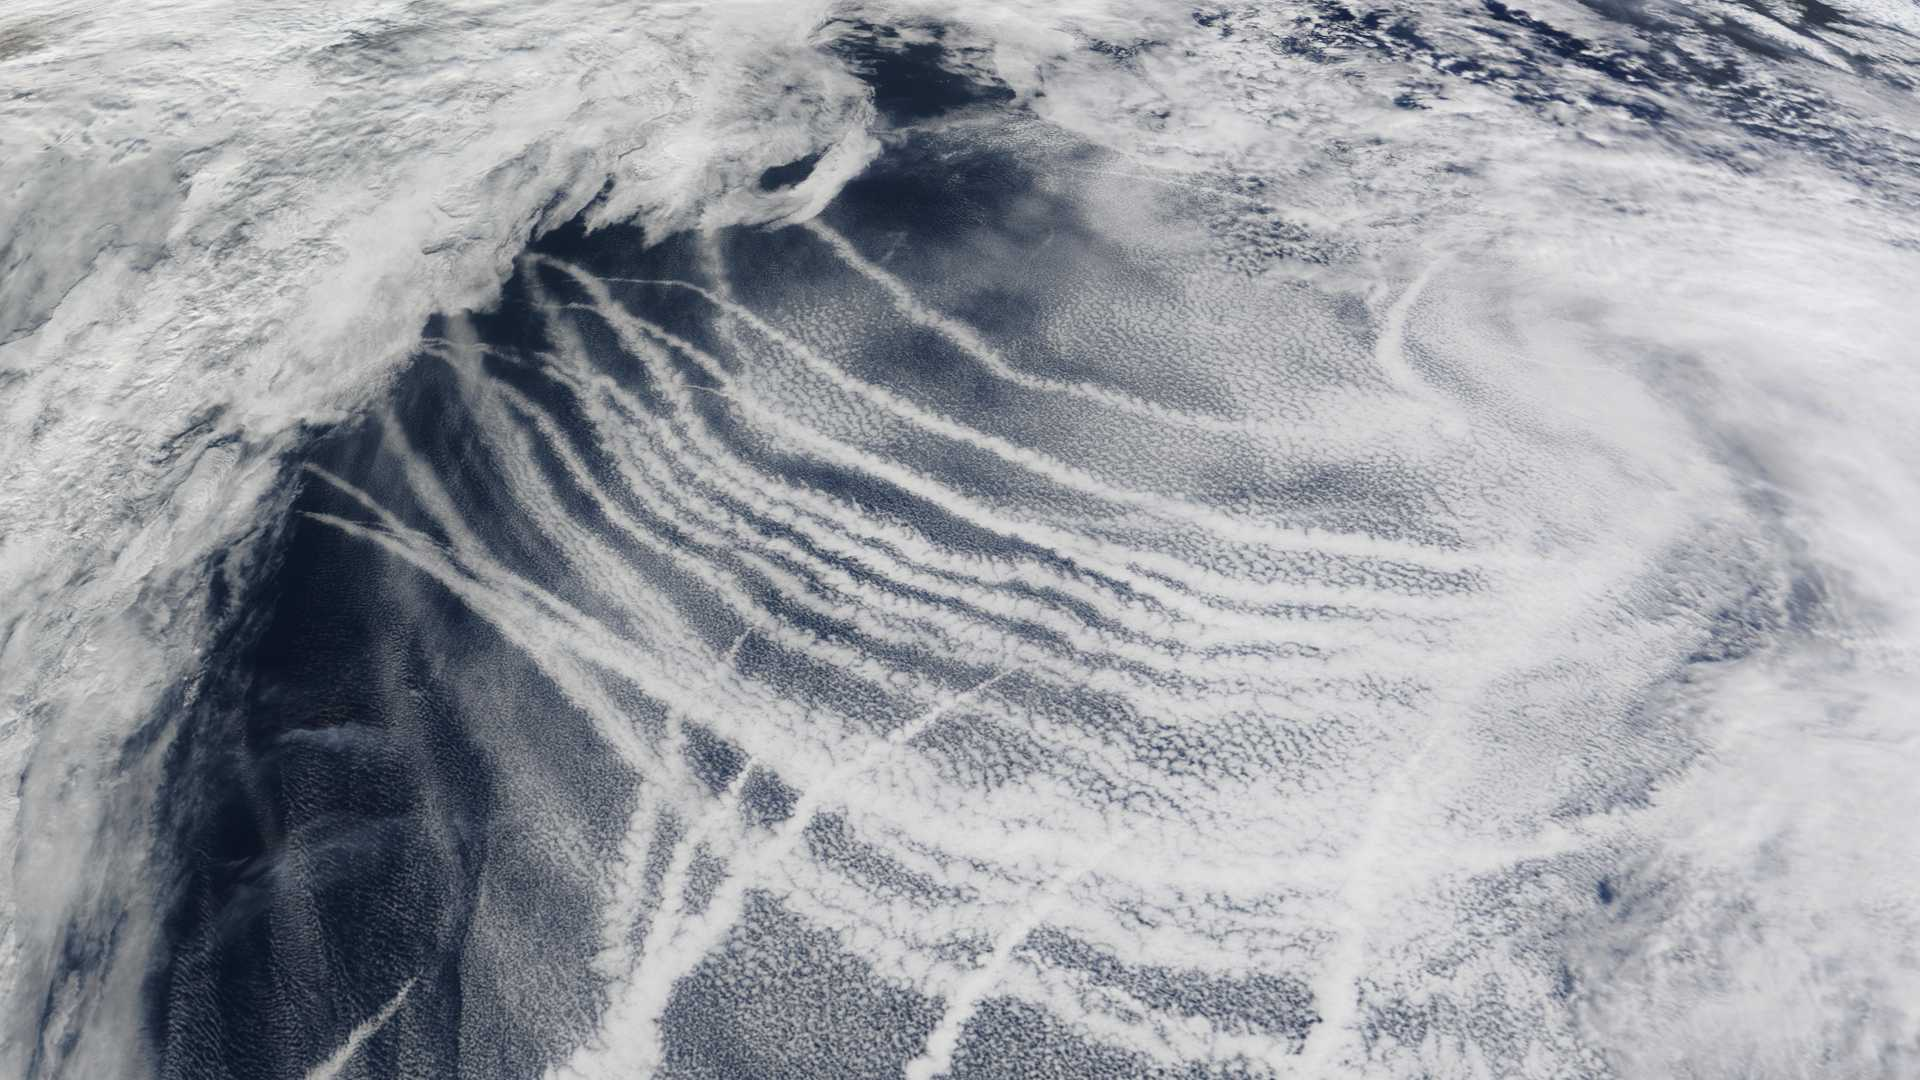
\includegraphics[width=0.65\textwidth]{figurer/ship_tracks.jpg}
\caption{\textit{Ship tracks observed by NASA's MODIS instrument on board the Aqua satellite. Figure retrieved from \url{https://svs.gsfc.nasa.gov/3667} October 9, 2019. More information about the instrument is found in Chapter \ref{ch:metode}.}}
\label{fig:shiptracks}
\end{figure}

\subsection{Subsection with reference}
\label{sec:ex:cite}

An example of a citation from a paper~\cite{glasius_composition_2018}.
	                % Scientific Background
\chapter[Research tools]{{\color{red}\fontsize 90 :}Research tools}
%
\label{ch:metode}
%

This chapter provides an overview of the model, satellite and reanalysis dataset applied in the thesis. Note that the work with preparing and analysing the satellite data in Paper III were performed by two other authors of the paper; Florent Malavelle and Jim Haywood. 

\section{NorESM}
\subsection{General information}
\subsection{OsloAero and AeroTab}

\subsection{Cloud treatment}

\subsection{Why NorESM?}


\section{ERA-Interim}
\subsection{General information}

\subsection{Why ERA-Interim?}


\section{MODIS-Aqua}
\subsection{General information}
\subsection{Why MODIS-Aqua?}




       % Instrumentation
\chapter[Presentation of findings]{{\color{red}\fontsize 90 :}Presentation of findings}
%
\label{ch:findings}
%

\section{Paper summary}\label{sec:paper:summary}



\subsection{Paper I: ''TITLE''}
\subsubsection{Objective}
\kant[10]
\subsubsection{Summary}
\kant[10]
\subsubsection{Author contribution}
\kant[10]

\subsubsection{Main findings}
\kant[10]
\begin{itemize}
\item \kant[11]
\item \kant[12]
\end{itemize}

\subsubsection{Main conclusion}
 \kant[13]
%%%%%%%%%%%%%%%%%%%%%%%%%%%%%%%%%%%%%%%%%%%%%%%%%%%%%%%%%%%%%%%%%%%%%%%%%

\newpage
\subsection{Paper II: ''TITLE''}

\subsubsection{Objective}
\kant[10]
\subsubsection{Summary}
\kant[10]
\subsubsection{Author contribution}
\kant[10]

\subsubsection{Main findings}
\kant[10]
\begin{itemize}
\item \kant[11]
\item \kant[12]
\end{itemize}

\subsubsection{Main conclusion}
 \kant[13]
%%%%%%%%%%%%%%%%%%%%%%%%%%%%%%%%%%%%%%%%%%%%%%%%%%%%%%%%%%%%%%%%%%%%%%%%%

%%%%%%%%%%%%%%%%%%%%%%%%%%%%%%%%%%%%%%%%%%%%%%%%%%%%%%%%%%%%%%%%%%%%%%%%%
\newpage
\section{Summary of answers to the sub objectives}\label{ch:subobj}
This section summarizes the specific answers to the sub objectives of the thesis.
\begin{enumerate}
\item \textbf{INSERT OBJECTIVE 1.}\\
  \kant[14]

        \item \textbf{INSERT OBJECTIVE 2.}\\
  \kant[14]


\end{enumerate}
  			% Summary of papers
\chapter[Discussion, future outlook and concluding remarks]{{\color{red}\fontsize 90 :}Discussion, future outlook and concluding remarks}
\label{ch:discussion}

\noindent TEXT


\section{Nudging}

\section{Historical changes impacting aerosol processes}

\subsection{Including historical oxidant changes}

\section{Rapid cloud adjustments}\label{ch:rapidcloudadj}


\subsection{Advances in recent years}

\subsection{Proposed solutions to remaining challenges}

\section{Concluding remarks and implications}
  			% Discussion

% Add bibliography to the table of contents
\addcontentsline{toc}{chapter}{Bibliography}
\bibliographystyle{bib/agufull08} %Two styles availabel in this template \bibliographystyle{bib/apacite}
\bibliography{bib/references}
%
\backmatter
 \fancyhf{}
 \renewcommand{\headrulewidth}{0pt} % and the line

% Include papers part
\part{Papers}
%
%\chapter*{Papers}
\label{ch:the_actual_papers}

%--------------------------------------------------------------------------------------------------
% Paper I
%--------------------------------------------------------------------------------------------------
\chapter*{Paper I}
\section*{TITLE }
%
\addcontentsline{toc}{chapter}{Paper I: TITLE}
%
\noindent Authors, authors, \textbf{CANDIDATE NAME}, authors authors \\
%
\noindent Geoscientific Model Development , 2018 \\
%
\noindent doi:10.5194/gmd-11-3945-2018
%
\begin{tikzpicture}[remember picture,overlay]
                \node[xshift=-1.3cm,yshift=-2.6cm] at (current page.north east)
{
\includegraphics[width=2cm]{decoration/paper1_red.pdf}};
\end{tikzpicture}

\cleardoublepage
%
\includepdf[pages=-]{papers/acp-19-4763-2019.pdf}

%--------------------------------------------------------------------------------------------------
% Paper II
%--------------------------------------------------------------------------------------------------
\chapter*{Paper II}
\section*{Strong impacts on aerosol indirect effects from historical oxidant changes}
%
\addcontentsline{toc}{chapter}{Paper II: TITLE}
%
\noindent \textbf{CANDIDATE NAME}, Jan Johansen etc \\
%
\noindent Atmospheric Chemistry and Physics , 2018 \\
%
\noindent doi:10.5194/acp-18-7669-2018

\begin{tikzpicture}[remember picture,overlay]
                \node[xshift=-1.3cm,yshift=-7.3cm] at (current page.north east)
{
\includegraphics[width=2cm]{decoration/paper2_red.pdf}};
\end{tikzpicture}

\cleardoublepage
%
%\includepdf[pages=-]{papers/paper2.pdf}


%--------------------------------------------------------------------------------------------------
% Paper III
%--------------------------------------------------------------------------------------------------
\chapter*{Paper III}
\section*{TITLE}
%
\addcontentsline{toc}{chapter}{Paper III: TITLE}
%
\noindent Authors \\
%
\noindent Nature , 2017 \\
%
\noindent doi:10.1038/nature22974
%
\begin{tikzpicture}[remember picture,overlay]
                \node[xshift=-1.3cm,yshift=-12.0cm] at (current page.north east)
{
\includegraphics[width=2cm]{decoration/paper3_red.pdf}};
\end{tikzpicture}

%
\cleardoublepage
%
%\includepdf[pages=-]{papers/paper3.pdf}

\cleardoublepage
%
%\includepdf[pages=-]{papers/paper3_suppl.pdf}

\cleardoublepage
%
%\includepdf[pages=-]{papers/paper3_erratum.pdf}

%--------------------------------------------------------------------------------------------------
% Paper IV
%--------------------------------------------------------------------------------------------------
\chapter*{Paper IV}
\section*{TITLE}
%
\addcontentsline{toc}{chapter}{Paper IV: TITLE}
%
\noindent \textbf{PHD CANDIDATE}, other authors \\
%
\noindent Journal of Geophysical Research - Atmospheres, \textit{in review} \\
%

%
\begin{tikzpicture}[remember picture,overlay]
                \node[xshift=-1.3cm,yshift=-16.7cm] at (current page.north east)
{
\includegraphics[width=2cm]{decoration/paper1_red.pdf}};
\end{tikzpicture}

%
\cleardoublepage
%
%\includepdf[pages=-]{papers/paper4.pdf}






% To include appendices
%
%\appendix
%\include{appendixA}             % Appendix A: Something
%
\end{document}
